\textbf{Stein, Shakarchi 3.13}

Suppose $f(z)$ is holomorphic in a punctured disc $D_r(z_0) \setminus \{z_0\}$, and that

$$
|f(z)| \le A|z - z_0|^{-1 + \epsilon}
$$

for some $\epsilon > 0$ and all $z$ near $z_0$. Show that the singularity of $f$ at $z_0$ is removable.

\begin{solution}
  If $\epsilon \ge 1$, then $f(z)$ is bounded near $z_0$ by $A$ for all $z$ in a sufficiently small open ball around 
  $z_0$ and so $z_0$ is a removable singularity by Riemann's theorem on removable singularities. We may therefore assume 
  $0 < \epsilon < 1$.  We proceed as in the proof of Riemann's theorem by defining $F: D_r \to \mathbb{C}$ of $f(z)$ to 
  be:

  $$
  F(z) = \frac{1}{2 \pi i} \int_C \frac{f(\zeta)}{\zeta - z} d\zeta
  $$

  where $C$ is the boundary of an open ball $B_R(z) \subset D_r(z_0)$ centered about $z_0$ such that the ball and its 
  boundary are entirely contained in the punctured disc; we fix $z \in B_R(z_0)$ with $z \neq z_0$, and utilize the 
  double keyhole contour shown in Figure \ref{fig:double_keyhole_contour} so that $F(z)$ is holomorphic on all of 
  $D_r(z_0)$ (that is, inside the contour and out) by a lemma from class. It remains to show that $F(z) = f(z)$ for all 
  $z \neq z_0$, which shows that $F$ is a holomorphic extension of $f$ and hence that the singularity of $f$ at $z_0$ is 
  removable. 

  \begin{figure}[h]
    \centering
    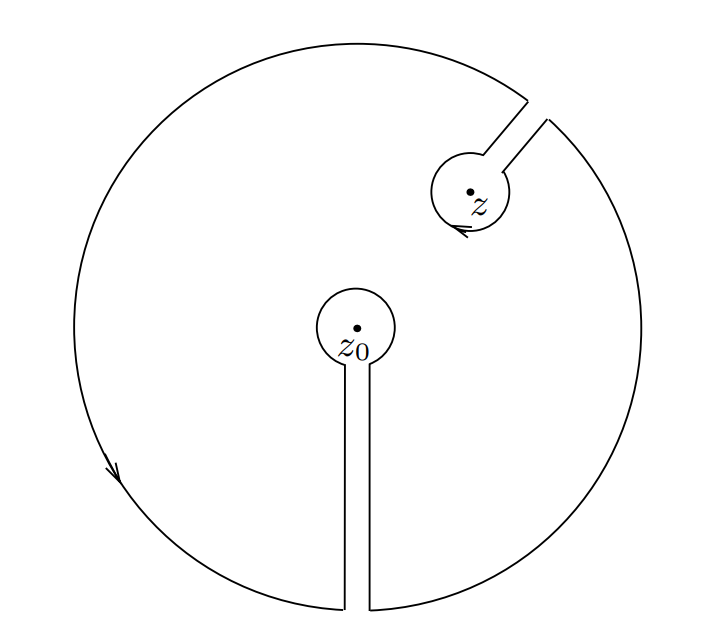
\includegraphics[width=0.4 \textwidth]{problem_7.png}
    \caption{Double keyhole contour.}
    \label{fig:double_keyhole_contour}
  \end{figure}

  We define $\gamma_0$ (resp. $\gamma$) to be a circle of radius $\delta_0$ (resp. $\delta$) centered about $z_0$ 
  (resp. $z$). Since $f(z)$ is holomorphic 
  in $D_r(z_0) \setminus \{z_0\}$, we can apply Cauchy's theorem to obtain (after letting the width keyhole corridors 
  cancel by tending toward zero):

  \begin{align*}
  0 &= \frac{1}{2 \pi i} \int_{C}{\frac{f(\zeta)}{\zeta - z} \; dz} 
     - \frac{1}{2 \pi i} \int_{\gamma_0}{\frac{f(\zeta)}{\zeta - z} \; dz}
     - \frac{1}{2 \pi i} \int_{\gamma}{\frac{f(\zeta)}{\zeta - z} \; dz} \\
    &= F(z) - \frac{1}{2 \pi i} \int_{\gamma_0}{\frac{f(\zeta)}{\zeta - z} \; dz} - f(z)
  \end{align*}

  where we have introduced negative signs for the latter two integrals since $\gamma$ and $\gamma_0$ have negative 
  orientation and used Cauchy's integral formula to simplify the third integral. We proceed to show that the remaining 
  integral vanishes, which proves the desired result. Firstly, we choose $\gamma_0$ small enough to be less than half 
  the distance between $z$ and $z_0$ so that along $\gamma_0$ (that is, $\zeta \in \gamma_0)$, we have 
  $|\zeta - z| \ge \frac{1}{2}|z_0 - z|$. Secondly, we choose $\delta_0$ small enough so that 
  $|f(\zeta)| \le A |\zeta - z_0|^{-1 + \epsilon}$. From these two inequalities, we obtain

  \begin{align*}
    \left| -\frac{1}{2 \pi i} \int_{\gamma_0} \frac{f(\zeta)}{\zeta - z} \right|
    &\le \frac{1}{2 \pi} \int_{\gamma_0} \frac{|f(\zeta)|}{|\zeta - z|} \; |d\zeta| \\
    &\le \frac{1}{2 \pi} \int_{\gamma_0} \frac{2 |f(\zeta)|}{|z_0 - z|} \; |d\zeta| \\
    &\le \frac{1}{\pi |z_0 - z|} \int_{\gamma_0} {A |\zeta - z_0|^{-1 + \epsilon}} \; |d\zeta| \\
    &= \frac{A \delta_0^{-1 + \epsilon}}{\pi |z_0 - z|} \int_{\gamma_0} {|d\zeta|}  \\
    &= \frac{A \delta_0^{-1 + \epsilon}}{\pi |z_0 - z|} 2 \pi \delta_0 \\
    &= \frac{2 A }{|z_0 - z|} \delta_0^{\epsilon} \\
  \end{align*}

  which vanishes in the limit as $\delta_0 \to 0$, as was to be shown.
  \ \\
\end{solution}